\section{Cel Projektu}
Celem projektu jest demonstracja możliwości zrównoleglenia obliczeń Szybkiej Transformaty Fouriera (FFT), na przykładzie przetwarzania obrazów.
\section{Wstęp}
\subsection{Technologia i zakres projektu}
\paragraph{Sposób działania programu}
Działanie programu polega na wczytywaniu obrazów w formacie BMP, poddawaniu ich
transformacji, a następnie zapisywaniu plików wyjściowych. Program dokonuje także transformacji odwrotnej. Możliwe jest zrównoleglenie poprzez uruchomienie kilku procesów (jeden proces na przetwarzanie jednego obrazu wejściowego) oraz skorzystanie z przetwarzania wielowątkowego. Działanie programu przetestowaliśmy na kilkunastu obrazach testowych o rozmiarach od $ 64x64 $ do $ 1024x1024 $.
\paragraph{Technologia i wykorzystane biblioteki}Program został napisany w C\#, do zrównoleglenia wykorzystujemy $ System.Diagnostics $ oraz $ System.Threading $.\\
 Pełna lista bibliotek:\\
 
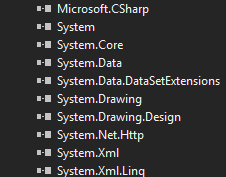
\includegraphics[scale=1]{figures/bibl.png}
\subsection{Wprowadzenie do tematyki FFT}

\paragraph{Zastosowania} Zastosowania transformacji obrazów to m. in.:
\begin{itemize}
	\item Uzyskanie bardziej zwartego (oszczędnego) sposobu kodowania obrazów
	(ich kompresji, np. standard kompresji obrazów JPEG),
	\item Uwidocznienie cech obrazu niezauważalnych w dziedzinie przestrzennej,
	np. zakłóceń okresowych.
\end{itemize}
\subsection{Szczegóły instalacji i uruchomienia programu} 
Po otrzymaniu pliku wykonywalnego \textbf{.exe} należy umieścić go w folderze, w którym znajduje się folder \textbf{img} a w nim obrazy, na których chcemy wykonać FFT. Obrazki muszą być w formacie \textbf{.bmp} oraz w zapisie 8bpp. 

Aby uruchomić program należy:
\begin{enumerate}
	\item Otworzyć \textbf{Wiersz poleceń (cmd)}
	\item Przejść do folderu z plikiem \textbf{.exe}
	\item Umieścić obrazy w folderze \textbf{img}, jeśli go nie ma należy taki utworzyć
	\item Uruchomić program z konsoli poleceniem:\\
	\textbf{\textit{FFT.exe [nazwa\_obrazka1] [nazwa\_obrazka1] [nazwa\_obrazka2] [nazwa\_obrazka3] [nazwa\_obrazka4]}}
	\subitem [nazwa\_obrazka] - to jest nazwa naszego obrazu bez rozszerzenia \textbf{.bmp}
	\subitem FFT.exe - zależy od tego czy zmieniliśmy nazwę pliku wykonywalnego, podana nazwa jest domyślna
	\item Dla każdego podane obrazka utworzył się w folderze \textbf{img} obrazek po FFT oraz po odwróconej FFT. (do nazw dodane przyrostki \textit{fourier} albo \textit{backwardfourier})
\end{enumerate} 
\section{Opis rozwiązania}

Zrównoleglenie przeprowadziliśmy poprze wprowadzenie wieloprocesowości oraz wielowątkowości.
\paragraph{Wieloprocesowość} Wprowadziliśmy możliwość uruchamiania przetwarzania każdego wczytywanego obrazu z linii poleceń na osobnym procesie.\\
	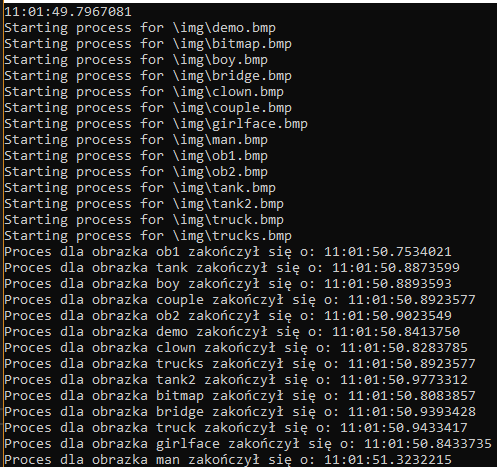
\includegraphics[scale=1]{figures/Par13Wat4.png}
\paragraph{Wielowątkowość} Podczas obliczeń FFT 2D należy wykonać transformatę najpierw na wierszach a następnie na kolumnach. Wykorzystaliśmy to, aby w zależności od ilości wątków definiowanych przez $THREADS$ przydzielać poszczególnym wątkom odpowiednią ilość wierszy, czy kolumn.\\
Należało zadbać o synchroniczny dostęp do tablicy $data$ podczas zapisu wyników częściowych.\\
\begin{lstlisting}
/**
* Moment of synchronization - lock for data table.
**/
 for (int j = 0; j < cols; j++)
	{
	lock(data)
		{
		 data[i, j] = row[j];
		}
	}
\end{lstlisting}
 
\clearpage\newpage

\clearpage\newpage

\section{Uzyskane rezultaty}
\begin{figure}[ht]
	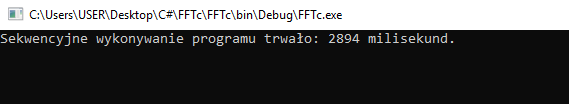
\includegraphics[width=\textwidth]{figures/Seq13.png}
	\centering
	\caption{Dla 13 obrazków 512x512 pikseli - wersja sekwencyjna}
\end{figure}
\begin{figure}[ht]
	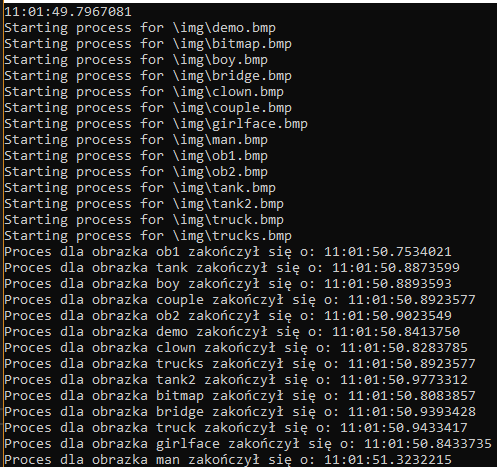
\includegraphics[width=0.8\textwidth]{figures/Par13Wat4.png}
	\centering
	\caption{Dla 13 obrazków 512x512 pikseli - wersja zrównoleglona 4 wątki}
\end{figure}
\begin{figure}[ht]
	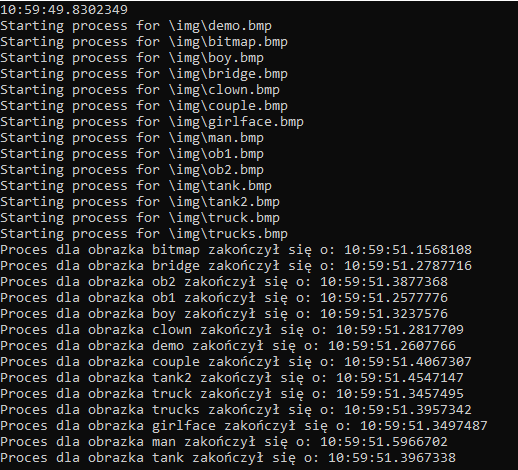
\includegraphics[width=\textwidth]{figures/Par13Wat8.png}
	\centering
	\caption{Dla 13 obrazków 512x512 pikseli - wersja zrównoleglona 8 wątków}
\end{figure}
\begin{figure}[ht]
	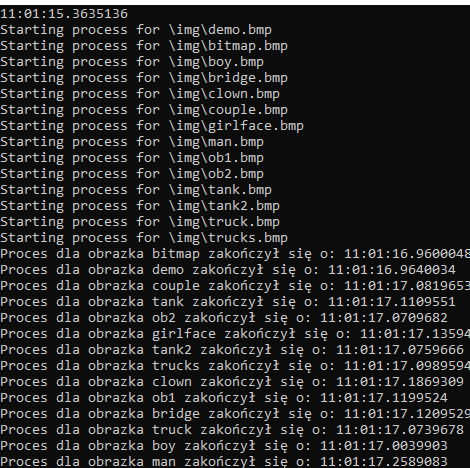
\includegraphics[width=\textwidth]{figures/Par13Wat16.png}
	\centering
	\caption{Dla 13 obrazków 512x512 pikseli - wersja zrównoleglona 16 wątków}
\end{figure}

\begin{figure}[ht]
	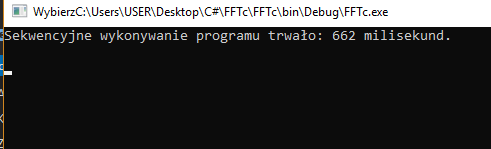
\includegraphics[width=\textwidth]{figures/Seq4.png}
	\centering
	\caption{Dla 4 obrazków 512x512 pikseli - wersja sekwencyjna}
\end{figure}
\begin{figure}[ht]
	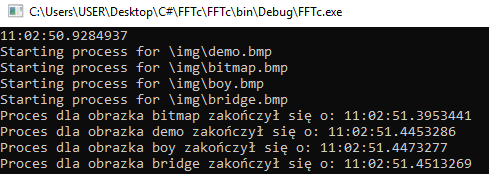
\includegraphics[width=\textwidth]{figures/Par4Wat8.png}
	\centering
	\caption{Dla 4 obrazków 512x512 pikseli - wersja zrównoleglona 8 wątków}
\end{figure}

\begin{figure}[ht]
	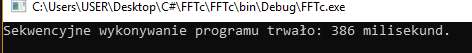
\includegraphics[width=\textwidth]{figures/Seq2.png}
	\centering
	\caption{Dla 2 obrazków 512x512 pikseli - wersja sekwencyjna}
\end{figure}
\begin{figure}[ht]
	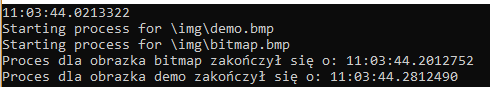
\includegraphics[width=\textwidth]{figures/Par2Wat8.png}
	\centering
	\caption{Dla 2 obrazków 512x512 pikseli - wersja zrównoleglona 8 wątków}
\end{figure}
\begin{figure}[ht]
	\centering
	%\caption{Podsumowanie}

	\begin{tabular}{@{}llllll@{}}
		\toprule
		Liczba obrazów & Liczba wątków & czas równolegle & czas sekwencyjnie & Przysp. w s & Przysp. \\ \midrule
		2              & 8             & 260             & 386               & 0,186              & 148\%          \\
		4              & 8             & 523             & 662               & 0,139              & 126\%          \\
		13             & 4             & 1527            & 2894              & 1,367              & 189\%          \\
		13             & 8             & 1766            & 2894              & 1,128              & 164\%          \\
		13             & 16            & 1895            & 2894              & 0,999              & 153\%          \\ \bottomrule
	\end{tabular}

\end{figure}
\clearpage\newpage
\section{Wnioski}
\begin{itemize}
	\item Po zastosowaniu transformaty w obie strony na obrazku zauważalny jest drobny spadek jakości obrazu.
	\item Zrównoleglenie na procesy poszeczególnych grafik dało bardzo dobre rezultaty i zdecydowanie przyśpieszyło działanie programu przy większej ilości obrazków.
	\item Wersja sekwencyjna jest równie szybka a czasami szybsza dla 2 lub 3 obrazków, ale od 4 i więcej zauważalna jest tendencja przyrostowa czasu wykonywania transformaty. W przeciwieństwie do zrównoleglonej wersji, gdzie czas utrzymuje się mniej więcej na tym samym poziomie.
	\item Użycie zbyt dużej ilości wątków wbrew pozorom daje gorsze rezultaty niż ich mniejsza ilość, np. 8 czy 4. Jest to spowodowane, że program traci czas na uruchomienie poszczególnych wątków, a one same w sobie nie mają dużego obciążenia obliczeniowego
\end{itemize}

